\subsection{Transistor}
\label{sec:transistor}

O transistor é o componente semicondutor fundamental da eletrônica moderna, utilizado para controlar o fluxo de corrente elétrica. Existem diferentes tipos de transistores, sendo os principais o transistor bipolar de junção (BJT) e o transistor de efeito de campo (MOSFET).

O BJT possui três terminais: emissor, base e coletor, sendo controlado por corrente. Já o MOSFET, amplamente utilizado em circuitos digitais, possui os terminais gate, source e drain, sendo controlado por tensão.

Em circuitos digitais modernos, especialmente em tecnologias CMOS, os transistores operam predominantemente como chaves (switches), conectando a saída ao nível lógico alto (Vcc) ou baixo (GND), dependendo do sinal de entrada.

\begin{figure}[H]
    \centering
    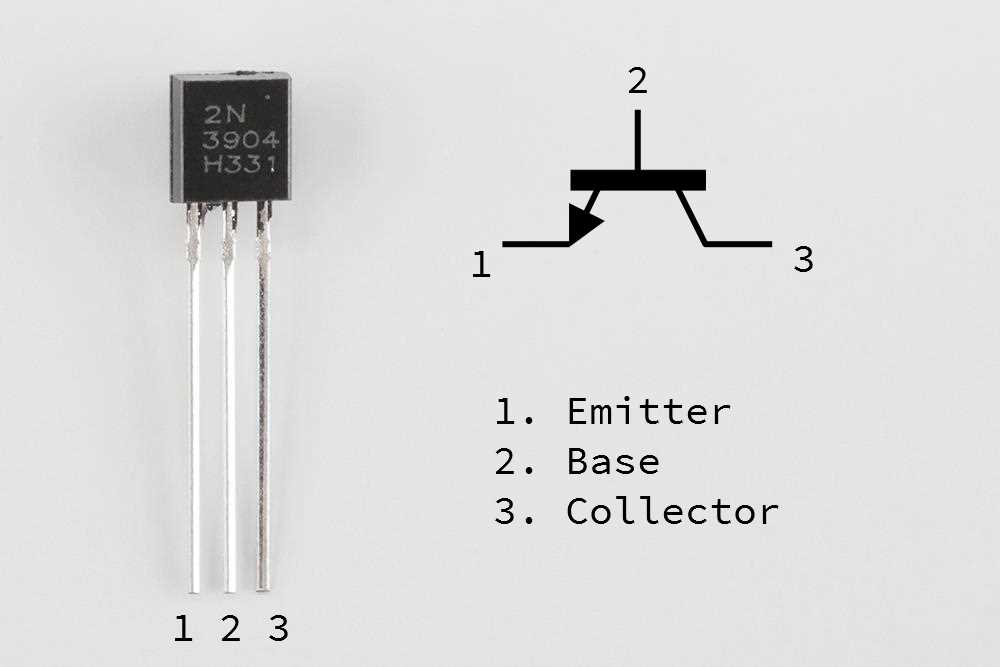
\includegraphics[width=0.6\linewidth]{images/transistor.jpg}
    \caption{Exemplo de transistor}
    \label{fig:transistor}
    {\footnotesize Fonte: \url{https://autoctrls.com/datasheet-transistor/}}
\end{figure}


\subsubsection{MOSFET tipo N e tipo P}

Os MOSFETs (Metal-Oxide-Semiconductor Field-Effect Transistors) são amplamente utilizados em circuitos digitais modernos e são controlados por tensão aplicada ao terminal gate.

Existem dois tipos principais:

\begin{figure}[H]
   	\centering
   	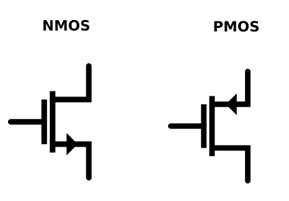
\includegraphics[width=0.6\linewidth]{images/NMOS-PMOS.jpg}
  	 \caption{MOSFET tipo N e tipo P}
   	\label{nmos-pmos-transistors}
	{\footnotesize Fonte: \url{https://www.langirswitch.com}}
\end{figure}

\begin{itemize}
    \item NMOS: conduz corrente quando a tensão no gate é alta (nível lógico 1). Nesse caso, o transistor conecta a saída ao nível lógico baixo (GND).
    
    \item PMOS: conduz corrente quando a tensão no gate é baixa (nível lógico 0). Nesse caso, o transistor conecta a saída ao nível lógico alto (Vcc).
\end{itemize}

Em circuitos CMOS (\textit{Complementaty Metal Oxide Semiconductor}), os transistores NMOS e PMOS são utilizados de forma complementar, permitindo maior eficiência energética e evitando consumo estático de corrente.


\subsubsection{BJT tipo NPN e PNP}

Os transistores bipolares de junção (BJT) são dispositivos controlados por corrente, possuindo três terminais: emissor, base e coletor.

Existem dois tipos principais:

\begin{figure}[H]
   	\centering
   	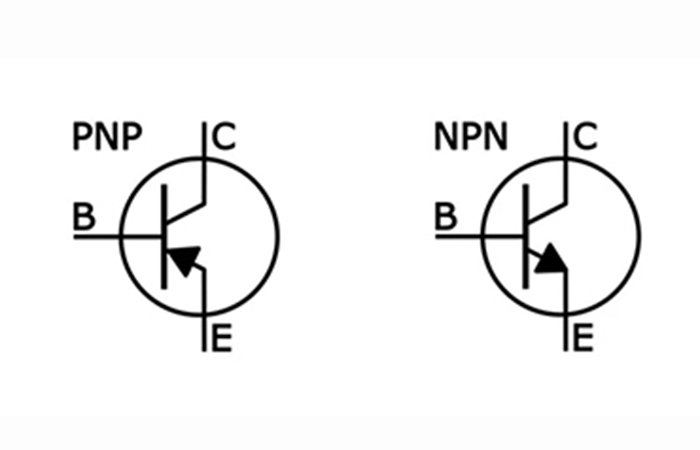
\includegraphics[width=0.6\linewidth]{images/npn-pnp-transistors.jpg}
  	 \caption{BJT tipo NPN e PNP}
   	\label{npn-pnp-transistors}
	{\footnotesize Fonte: \url{https://www.langirswitch.com}}
\end{figure}

\begin{itemize}
    \item {NPN}: conduz corrente entre coletor e emissor quando há corrente entrando na base. É ativado por um sinal positivo na base em relação ao emissor.
    
    \item {PNP}: conduz corrente quando há corrente saindo da base. É ativado por um sinal negativo na base em relação ao emissor.
\end{itemize}

Diferentemente dos MOSFETs, os BJTs exigem corrente contínua na base para se manterem ativos, o que os torna menos eficientes para aplicações digitais modernas.
